\chapter{Software Defined Radio}



\section{USRP}

The USRP (Universal Software Radio Peripheral) is intended to provide a 
low-cost, high quality hardware platform for software radio. It is designed
and marketed by Ettus Research, LLC. It is commonly used by research labs,
universities, and hobbyists. The USRP platform is designed for RF applications
from DC to 6 GHz. USRPs connect to a host computer through a high-speed USB or
Gigabit Ethernet link, which the host-based software uses to control the USRP
hardware and transmit/receive data.

The USRP Hardware Driver (UHD) is the official driver for all Ettus Research
products. The UHD supports Linux, Mac OS X and Windows.

\begin{figure}
\centering
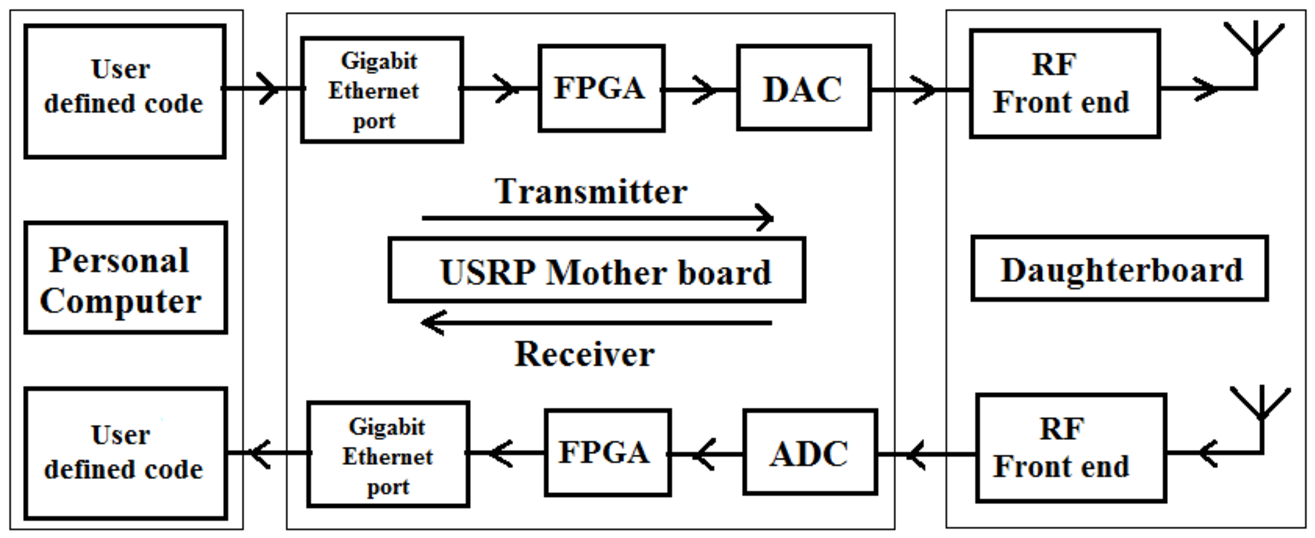
\includegraphics[width=0.7\textwidth]{usrpBlock}
\caption[Block diagram of USRP]{Block diagram of USRP.\\
\emph{Source:\\ Kranthi Ananthula, Experimental setup of Cognitive Radio 
Test-Bed using Software Defined Radio, M. Tech. Dissertation, 2013.}}
\label{usrpBlock}
\end{figure}

In this project we are using a particular model of USRP product known as the
USRP N210.

\subsection{USRP N210}

The USRP N200 and N210 are the highest performing class of hardware of the 
USRP family of products, which enables engineers to rapidly design and 
implement powerful, flexible software radio systems. The N200 and N210 
hardware is ideally suited for applications requiring high RF performance and
great bandwidth. Such applications include physical layer prototyping, dynamic
spectrum access and cognitive radio, spectrum monitoring, record and playback,
and even networked sensor deployment. The Networked Series products offers 
MIMO capability with high bandwidth and dynamic range. The Gigabit Ethernet
interface serves as the connection between the N200/N210 and the host 
computer. This enables the user to realize 50 MS/s of real-time bandwidth in 
the receive and transmit directions, simultaneously (full duplex).


\section{GNU Radio}

\subsection{Introduction}
GNU Radio is a free \& open-source software development toolkit that provides 
signal processing blocks to implement software radios. It can be used with 
readily-available low-cost external RF hardware to create software-defined 
radios, or without hardware in a simulation-like environment. It is widely 
used in hobbyist, academic and commercial environments to support both 
wireless communications research and real-world radio systems.

\subsection{What does GNU Radio do?}
It does all the signal processing. You can use it to write applications to 
receive data out of digital streams or to push data into digital streams, 
which is then transmitted using hardware.

GNU Radio has software equivalents of real world radio system components like 
filters, demodulators, equalizers, etc. These are usually referred to as
blocks. You can create a complex system by connecting various blocks. If you
cannot find some specific blocks, you can even create your own blocks and add
them.

Most of GNU Radio has been implemented using the Python programming language,
and the performance-critical parts have been implemented using C++. Typically,
a GNU Radio user writes his applications in Python, unless he has some
performance-critical needs. Thus, GNU Radio gives its users an easy-to-use,
rapid application development environment.

\subsection{GNU Radio with USRP}

\begin{figure}[h]
\centering
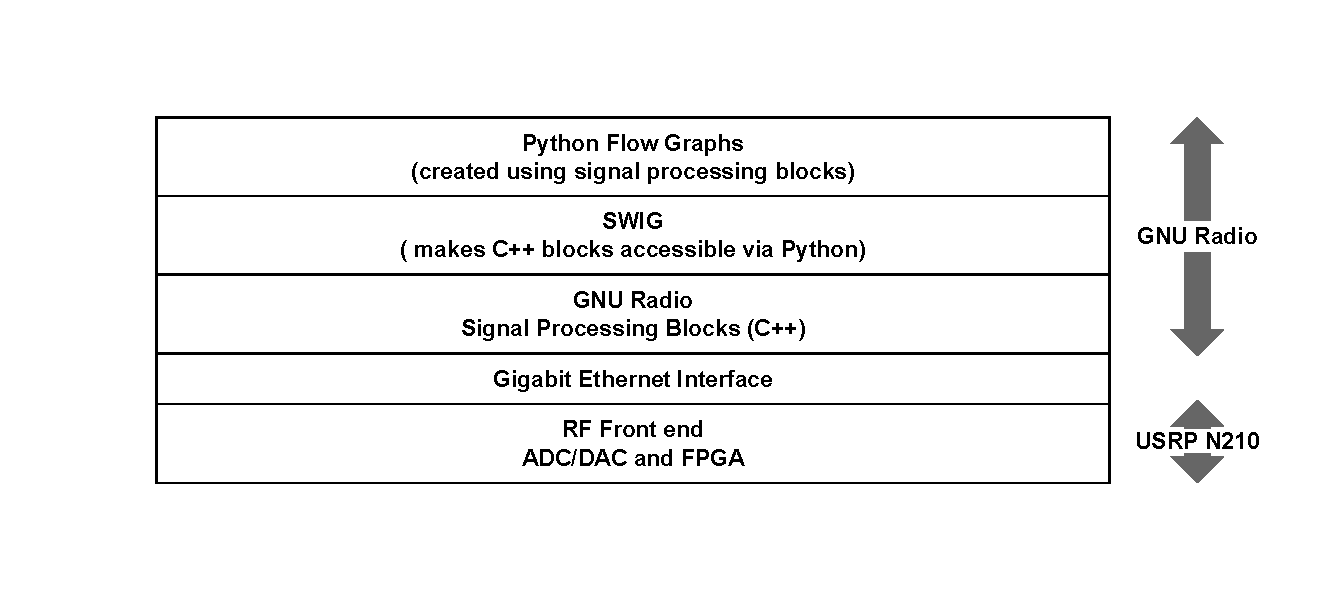
\includegraphics[width=0.9\textwidth]{gnuradio_architecture}
\caption{Architecture of GNU Radio}
\label{gnuradio_architecture}
\end{figure}

The USRP and the host computer make up the hardware part of the SDR system. 
The host computer must run a compatible software package such as GNU Radio or
Simulink to complete the SDR system. In this project we are using GNU Radio
as the software platform.

GNU Radio communicates with the USRP through the USRP Hardware Driver (UHD)
software. The UHD provides a host driver and an Application Programming
Interface (API) for the USRP. GNU Radio uses the UHD to set user-specified
parameters like RF center frequency, antenna selection, gain, sampling rate,
interpolation, decimation, etc.

